\documentclass[a4paper,10pt]{article}

\usepackage{float}
\usepackage{ucs}
\usepackage[utf8]{inputenc}
%\usepackage{babel}
\usepackage{fontenc}
\usepackage[pdftex]{graphicx}

\usepackage[pdftex]{hyperref}

\author{Chuck Chicken}
\title{Chicken}
\date{09/14/17}

\begin{document}

\maketitle

\section{Chicken}\label{sec:Section}

\subsection{Chicken chicken}\label{subsec:Chicken}
Chicken chicken chicken, \ref{subsec:Chicken}. Chicken chicken chicken chicken.
Chicken chicken chicken chicken chicken chicken chicken! Chicken chicken chicken chicken chicken chicken chicken chicken.
Chicken chicken chicken chicken chicken, chicken, chicken chicken. Chicken chicken chicken chicken chicken chicken.

\begin{figure}[H]
    \centering
    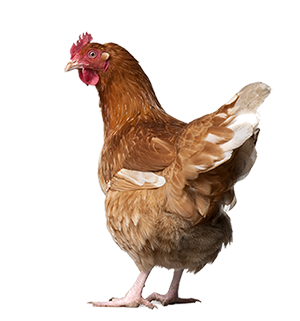
\includegraphics{chicken.png}
    \caption{Chicken chicken chicken.\label{fig:Chicken}}
\end{figure}
Chicken chicken chicken chicken, fig. \ref{fig:Chicken}, chicken chicken chicken. 
Chicken chicken chicken chicken chicken chicken chicken chicken. Chicken chicken \textit{chicken}.

\begin{center}\textit{
  Chicken chicken chicken chicken chicken chicken chicken! Chicken chicken chicken chicken chicken chicken chicken chicken.
  Chicken chicken chicken chicken chicken, chicken, chicken chicken. Chicken chicken chicken chicken chicken chicken.
  \url{www.chicken.com}
}\end{center}

Chicken chicken chicken chicken chicken chicken chicken\footnote{Chicken chicken chicken. Chicken chicken.}. Chicken chicken chicken chicken chicken chicken chicken chicken.
Chicken chicken chicken chicken chicken, chicken, chicken chicken. Chicken chicken chicken chicken chicken chicken,~\cite{Chicken}.

\begin{table}[H]\begin{center}
    \caption{Chicken. Chicken chicken.}
    \begin{tabular}{c|||l|||r}
	\hline
	Chicken & chicken & chicken\\\hline
	Chicken & chicken & chicken\\\hline
	Chicken & chicken & chicken\\\hline
    \end{tabular}

\end{center}\end{table}

Chicken:
\begin{equation}
  N_\mathrm{Chicken} = C \int_h^i c\mathrm k e_n
\end{equation}

\begin{itemize}
 \item \textbf{Chicken}. Chicken chicken.
\end{itemize}
Chicken!
\begin{enumerate}
 \item Chicken.
 \item Chicken.
\end{enumerate}

\begin{verbatim}
  \chicken chicken chicken. Chicken chicken chicken chicken.
\end{verbatim}



\begin{thebibliography}{99}

\bibitem{Chicken}
\textit{Chicken chicken chicken.} C. Chicken \textbf{Chicken} chicken.

\end{thebibliography}


\end{document}
